
% Many thanks to Andrew West for writing most of this file
% Main LaTeX file for CIS400/401 Project Proposal Specification
%
% Once built and in PDF form this document outlines the format of a
% project proposal. However, in raw (.tex) form, we also try to
% comment on some basic LaTeX technique. This is not intended to be a
% LaTeX tutorial, instead just (1) a use-case thereof, and (2) a
% template for your own writing.

% Ordinarily we'd begin by specifying some broad document properties
% like font-size, page-size, margins, etc. -- We have done this (and
% much more) for you by creating a 'style file', which the
% 'documentclass' command references.
\documentclass{sig-alternate}
 
% These 'usepackage' commands are a way of importing additional LaTeX
% styles and formattings that aren't part of the 'standard library'
\usepackage{mdwlist}
\usepackage{url}
\usepackage{float}
\usepackage{listings}

\begin{document} 

% We setup the parameters to our title header before 'making' it. Note
% that your proposals should have actual titles, not the generic one
% we have here.
\title{Programming Language Support for Probabilistic Associative Memory}
\subtitle{Dept. of CIS - Senior Design 2014-2015\thanks{Advisor: Steve A. Zdancewic (stevez@cis.upenn.edu).}}
%\thanks{ Do not list your advisors amongst the authors as that may cause Google Scholar to add this work to their list of publications. Your advisor must also sign a hard-copy of your proposal.}}
%\thanks{ }}
\numberofauthors{3}
\author{
    Fan Yin \\ \email{fanyin@seas.upenn.edu} \\Univ. of Pennsylvania \\ Philadelphia, PA
    \and Haolin Lu \\ \email{haolinlu@seas.upenn.edu} \\Univ. of Pennsylvania \\ Philadelphia, PA
    \and Yukuan Zhang\\ \email{yukuan@seas.upenn.edu} \\Univ. of Pennsylvania \\ Philadelphia, PA
}
%\author{
%\alignauthor Radoslav Ivanov \\ \email{rivanov@seas.upenn.edu} \\ Univ. of Pennsylvania \\ Philadelphia, PA 
%
%\and Radoslav Ivanov \\ \email{rivanov@seas.upenn.edu} \\ Univ. of Pennsylvania \\ Philadelphia, PA 
%
%}
\date{}
\maketitle

% TODO: don't mention ocaml except in system implementation.
% TODO: get rid of "we"?

% Next we write out our abstract -- generally a two paragraph maximum,
% executive summary of the motivation and contributions of the work.
\begin{abstract}
    Our goal is to create a programming language library that provides an interface
    for programming with a probabilistic associative memory.
    A probabilistic associative memory receives an input and returns a value associated with
    or similar to the input. This project provides an intuitive interface to this probabilistic
    associative memory to facilliate programming efficiency for the end user. It will primarily
    accomplish this by providing an easier way to handle structured input data for the user, as well
    as automatically managing user-defined types in memory.
\end{abstract}

\section{Background}
\label{sec:intro}

The standard way to access a stored value in memory is by address. 
This involves finding the physical position of that address in memory
and returning the stored value. Meanwhile, associative memory allows
searching for values based on the stored content. An analogous structure
in programming languages is the hashtable, which returns an output value
based on an input key. 

Standard associative memories are useful for when one needs to query memory based 
on some input data or tag. For instance, router firmware often employs associative 
memories to store tables of Internet Protocol (IP) addresses, which serve as the ``next hop" for incoming 
packets. Since routers looking for the ``next hop" have a specific, standard query 
format -- e.g. an IP address of the form www.xxx.yyy.zzz -- it makes sense to store the 
routing tables based around this input string.

Probabilistic associative memories retain the content-based characteristics of associative memories.
However, they stop maintaining the discrete one-to-one relationship between input and output.
A modern day realization of probabilistic associative memories is the neural network. A neural network
consists of a series of functions acting on ``features" or characteristics of given input values. Using
these functions, it can find relationships or make predictions on its inputs. It also
reacts and changes whenever it sees new input to enhance accuracy for future input.

Neural networks are a small part of the much broader topic of \textbf{machine learning}. Machine learning
is widely used today to solve problems that lack easily definable patterns (i.e. natural language processing,
computer vision, classification). A common feature of these problems is that they usually have a large amount
of sample data available. The goal of machine learning algorithms is to build models based on an
abundant amount of ``training data". Since the types of data vary wildly from one problem to the next,
from sentences in several languages to video data from a camera, a way to reconcile the data with
mathematical models is required. In this respect, ``feature extraction" is essentially the de facto
standard for a majority of machine learning algorithms. Feature extraction involves transforming the
input data into a vector of real numbers, while trying to encapsulate as much of the information
in the original data as possible. These vectors are then run through the model to improve accuracy,
acquire a result, or both. See figure 1 for a representation of this process. 
Machine learning ideas and techniques will be crucial to this project,
as they will be used as the foundation of the memory system, as well as being the area where this project
will have the biggest impact.

%TODO: reference to figure 1...update?

%Since our queries work directly with a probability model, it would offer more fluidity
%with programming that involves statistical modeling or simulations. 
%Returning values based on a probability also saves memory because not every value has to be stored. 
%In a simplistic representation of a probability model, a frequency table of memory values can be constructed as memory values are stored.
%The queries would then consist of a set of values, and a likelihood would be generated based on both frequency and some matching metric in that query-set.
%Thus, the memory mechanism can extrapolate or interpolate a response to a query based on values 
%previously inserted into memory. 

%See Figure 1 for a representation of the flow of this probabilistic mechanism.
\begin{figure}[H]
	\begin{center}
		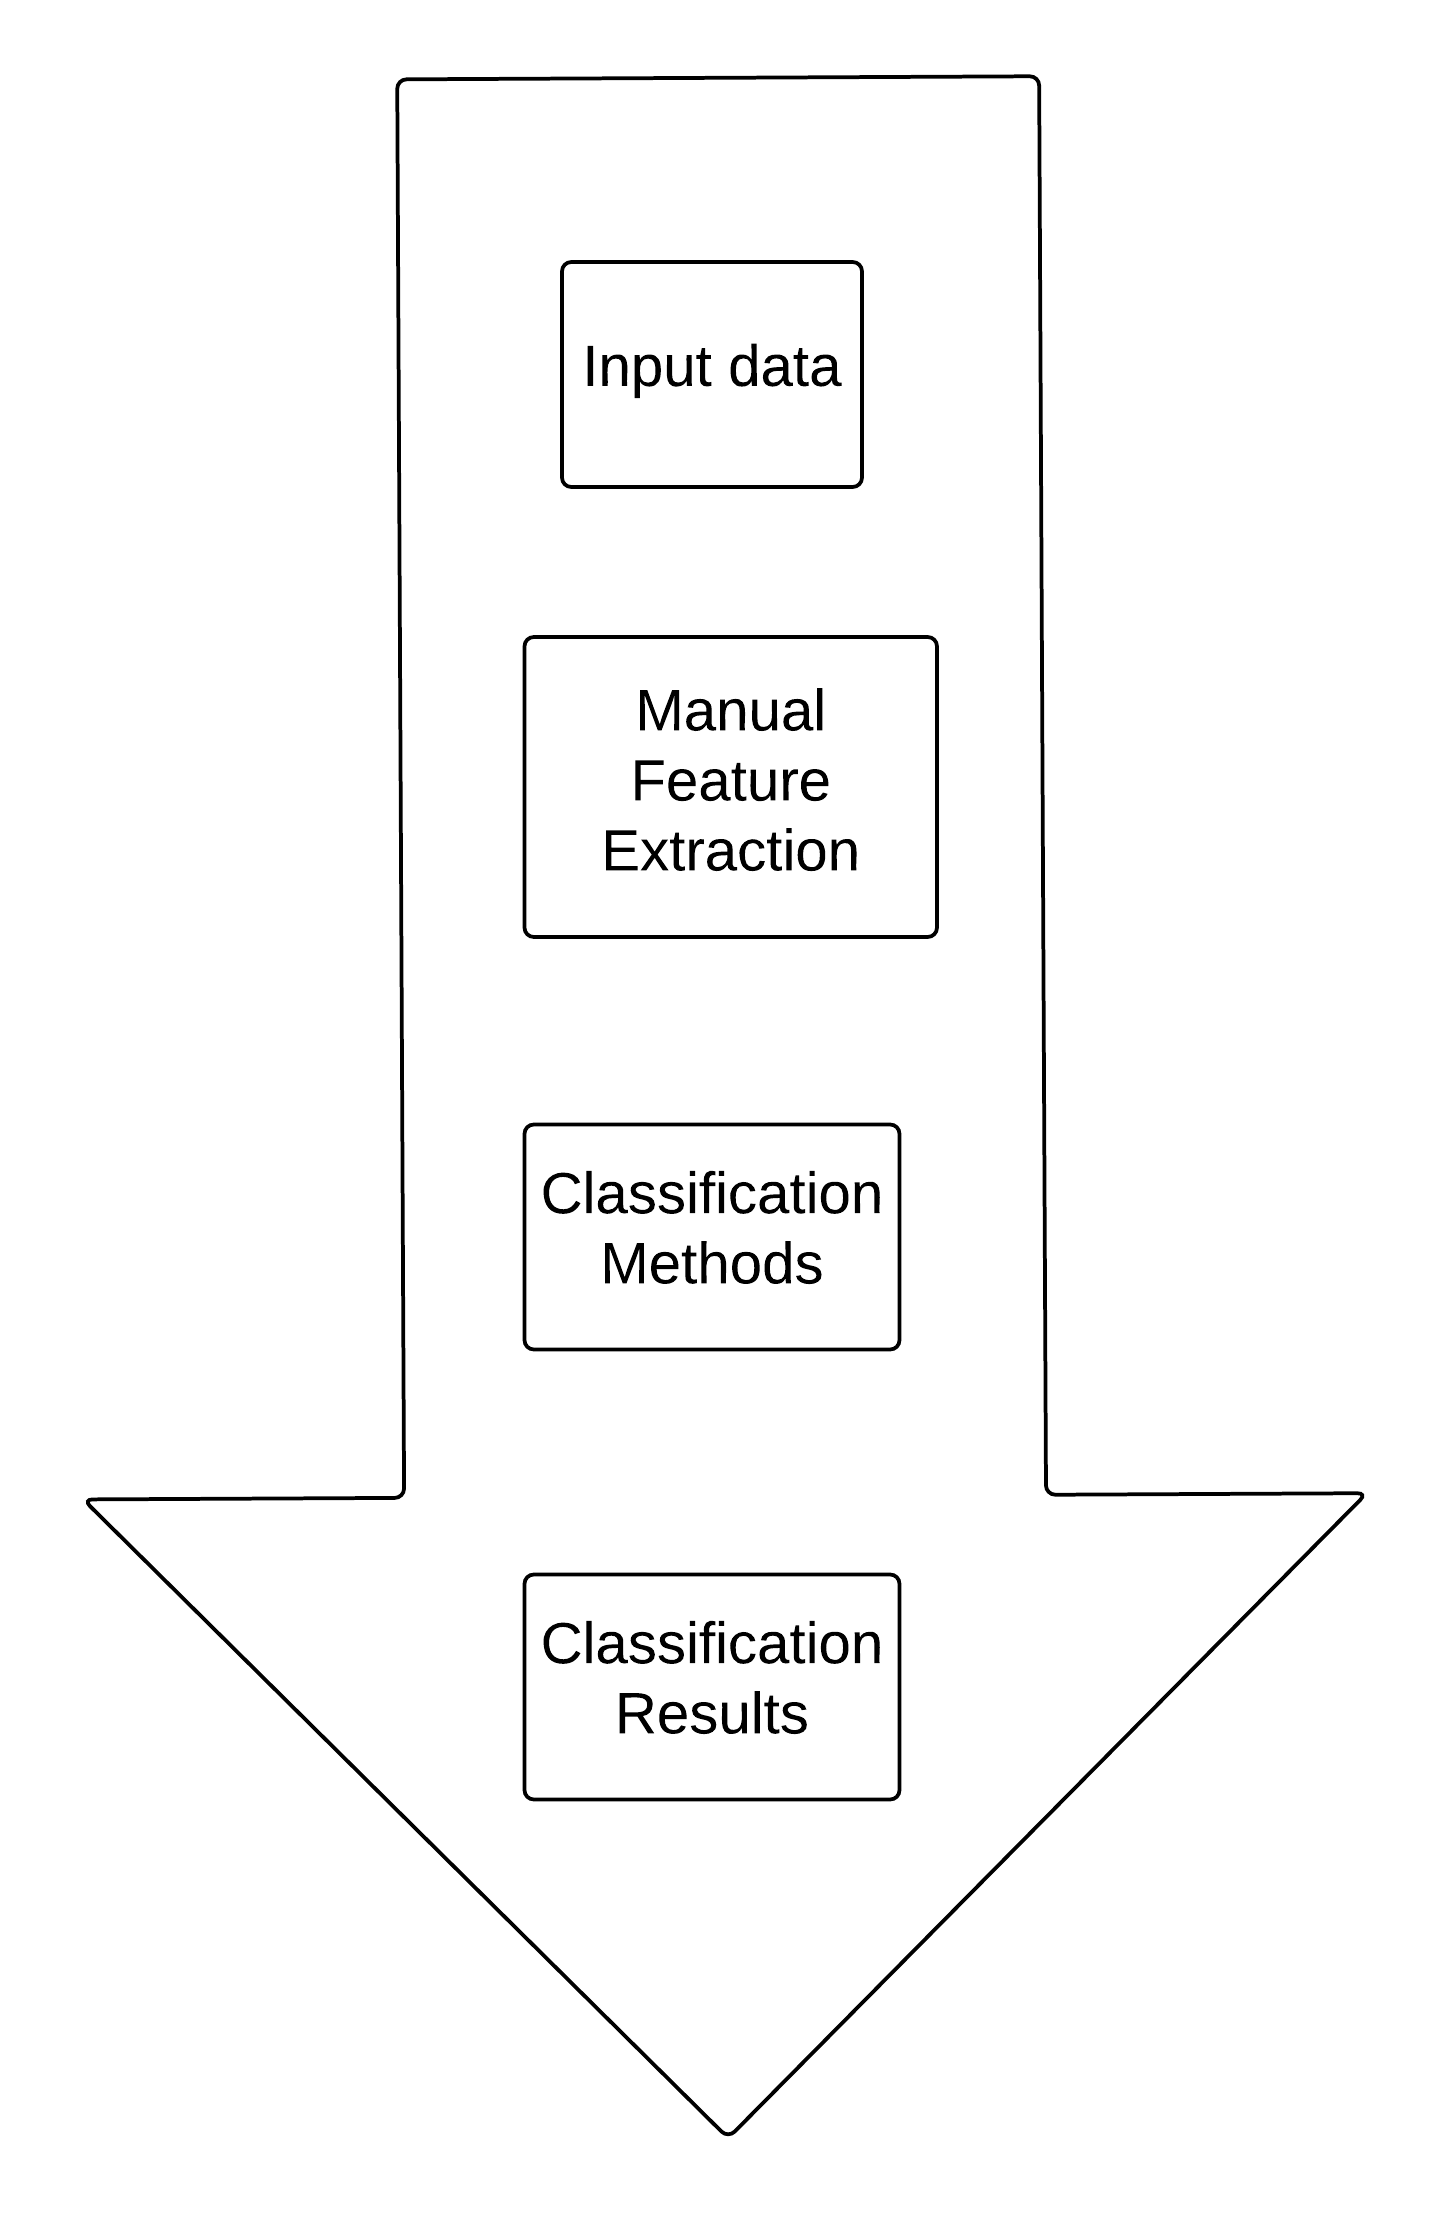
\includegraphics[width=0.75\linewidth]{mlworkflow}
	\end{center}
	\vspace{-12pt}
	\caption{Model of Standard Machine Learning Workflow}
	\label{fig:mlworkflow}
\end{figure}


%The implementation may also include support for structured data in the probabilistic associative memory.
%In a standard associative memory scheme, a similarity query is done by comparing input bits
%to the values stored in memory. However, this does not allow for accurate similarity comparisons
%between trees or lists, as the memory is not aware of the underlying structure. As a result,
%many applications on structured data will first flatten the structure, perform the requisite 
%calculations, then reconstruct the original structure of that data. With a built-in type system
%that supports structured data, the user will be able to directly manipulate the data in memory 
%while keeping the structure intact.

%Practical applications of probabilistic associative memories involve various approximation and prediction methods.
%These involve appliactions such as image reconstruction from noisy input data, or search autocompletion.
%This project strives to provide a simple, flexible interface to work with these probabilistic associative memories.

%TODO 
%FIGURE: Standard flow for ML 
%Training data --> manually convert into feature vectors --> run vectors through classifier algorithms/models --> get classification results/decisions

\section{Introduction}
\label{sec:intro}

In machine learning, the issue of feature extraction is dependent upon
the type and structure of the data. Whether the input data set is 
represented as lists, pairs, trees, or another type of data structure will 
have a huge impact on how feature extraction will occur. 

So far, we have investigated various methods of handling this issue with structured data, 
Since we intend to apply our extraction methods on top of our probabilistic
associative memory, we have also begun working on the memory backend of our
library interface. It is necessary to introduce the autoencoder and kernel 
methods to further elaborate on this: Autoencoders are neural networks that
take in a set of data and return a reduced, compressed representation of that
data. That is, it returns an encoding. This is akin to feature extraction, 
since the whole concept of feature extraction is finding the essential features 
of a set of data. Kernel methods, on the other hand, are a way of projecting
a set of data in one space to another space, with the intention that it may
be easier to extract essential data in the latter space.

What must still be done is integrating these two methods with our library.
As will be detailed later, there has been research done on linear autoencoders
for structured data, and there has also been previous work on convolution 
kernels for natural language processing -- a field that processes a lot of 
data in the form of structured trees. What will be done is to better understand
the mathematical machinery behind autoencoders and kernel methods, and to
implement those methods in our library.

% TODO: get rid of 'probabilistic' here if we're getting rid of that in related work
% TODO: get rid of any mentions of performance here if we're not really talking about that later
In the next section, the paper will proceed by delineating works related to 
probabilistic associative memory and will go more in-depth about autoencoders 
and convolution kernels. Then, it will establish a model or workflow of the 
library interface, and the process of using this interface for a machine
learning application. After that, it will go into some details of the library
implementation, and discuss our choice of language -- OCaml -- and some third-
party libraies we used. Finally, we will discuss the performance of our current
implementation, as well as the remaining work that must be done.

\section{Related Work}
\label{sec:related_work}

With regards to existing related work, the goal of this project is not to advance associative memory 
techniques. Rather, it is seeking to research existing models for associative memories, provide a 
simple probabilistic query interface, and integrate a method of extracting essential features from 
the structured data that is input into the memory. With that in mind, there are many works that 
address associative memory and feature extraction from structured data.

Research in associative memory has close connections to neural networks. Our brains function as 
associative memories that can retrieve memories based on similarity between stimuli and the memories 
themselves.  Indeed, Norman and Bobrow~\cite{bobrow} construct a memory model which describes how 
minds retrieve items in memory from partial descriptions, even if some part of the description is 
incorrect or inaccurate. 

Applying this memory model to computation, Hinton~\cite{hinton} draws a connection between Norman 
and Bobrow's idea of retrieving memories based on partial descriptions and content-addressable 
memories.  Hinton then notes that although this content-addressable memory is a useful 
representation, it is difficult to efficiently ``search for content" through a memory space. 
Hinton ends by claiming that while this model is conceptually not difficult, it is difficult to 
actually implement it. He mentions that an approach to this problem that has arisen recently is with 
stochastic processes -- heralding a probabilistic approach to this associative memory problem.

To address the issue of increasingly large data sets, resulting in larger and larger feature vectors,
much research has been made to decrease dimensionality of feature vectors. One such modern technique
is the autoencoder. Researchers Hinton and Salakhutdinov %cite
describe a method of creating deep autoencoders to learn low dimensionality codes that maintain
high fidelity with respect to codes of the original dimension.

An extension of classic autoencoders called a denoising autoencoder has the ability to reconstruct 
partially missing or corrupt inputs. This property of denoising autoencoders make them extremely 
promising for use in a memory system. Denoising autoencoders work by passing input through a hidden 
layer, a matrix that represents a transformation, to encode it in a lower dimension. The original 
input is then ``retrieved" by doing a reverse transformation on the encoded version. 

%TODO: structured data and convolution kernels

% possibly implementation
Notice that as the dimension
of the hidden layer increases, the optimal transformation matrix approaches the identity, since
the identity matrix is the best possible representation if the hidden layer had the same dimension
as the input. To create useful representations even in these situations, the autoencoder is trained
by intentionally corrupting the input, passing it through the autoencoder, and doing a gradient
descent on the error between the output and the original input.

\section{System Model}
\label{sec:sysmodel}

%TODO: remember to change figure numbers

%FIGURE: Standard flow for this library implementation
\begin{figure}[H]
	\begin{center}
		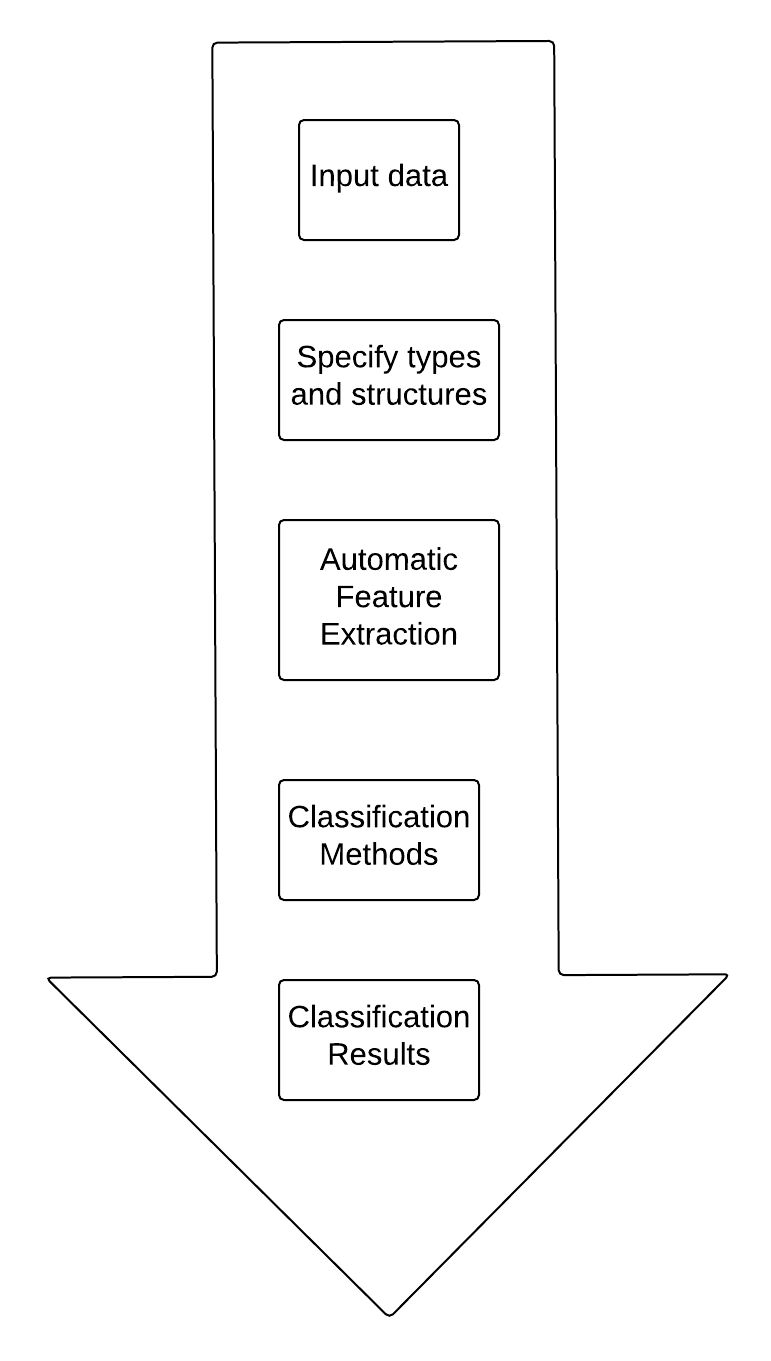
\includegraphics[width=0.75\linewidth]{ourworkflow}
	\end{center}
	\vspace{-12pt}
	\caption{Library Interface Workflow as Applied to Machine Learning}
	\label{fig:ourworkflow}
\end{figure}

%TODO: talk more about the memory?
%TODO: clean up ML part?
Figure 2 shows a model of the workflow of using this programming library. In similar fashion to 
standard machine learning applications, the user will start with a set of training data which can 
take various structures such as trees or lists. The user will then need to specify the type and 
structure of the data he is inputting to the library, so the library will know how to process it 
appropriately. Regarding this data specification, the user will do this implicitly when he processes 
his sample data and loads it into custom types defined by the library or by OCaml itself. 
Next, the library will use an algorithm or model to actually perform this feature extraction. In 
comparison to the standard machine learning workflow in figure 1, the workflow when using this 
library will provide automatic feature extraction, as opposed to requiring the programmer to 
manually extract the feature through his own custom code.  The rest of the library after feature 
extraction will more or less proceed according to standard machine learning methods.
That is, the library will run the vectors through classification algorithms and models 
and return the classification results or decisions.

From our research, we have investigated methods that handle ``automatic" feature extraction, given
the data type or structure. To reiterate, convolution kernel methods and linear autoencoder networks 
could accomplish this extraction over various structures of data. These methods have been tested and 
applied to NLP applications and classification problems involving data stored in trees and sequences.
Thus, the approach of this library should at least work for any sort of tree-like or list-like 
structure.

\section{System Implementation}
\label{sec:sysimp}

%TODO: how much do we want to talk about blas/lapack here?
In order to implement a generalized process for handling structured data, the programming language 
library has been written in OCaml. OCaml is a functional language, so it will be more elegant and 
efficient to use when handling structured data. That is, eventually, the library will have the 
capability to handle custom, user-defined data types, and creating a user-defined type in OCaml is a 
more fluid process than it would be in procedural languages. OCaml, however, is not as purely 
functional as languages such as Haskell. It has procedural elements that facillitates the ease of 
implementing and prototyping the various algorithms and models that we have researched. In addition, 
there is a linear algebra for OCaml called Lacaml that uses BLAS and LAPACK as its backend, which 
are two well-established, robust and performant linear algebra libraries.

\section{System Performance}
\label{sec:sysperformance}

The portion of the library that can be measured so far is the basic autoencoder model. 
Since it is based on a reference implementation, we can compare performance statistics of both
implementations. Due to randomization inherent in the algorithm though, performance must be
standardized by either choosing the same random initialization parameters, or averaging 
across multiple runs. 

The latter was not possible due to performance issues in the current implementation. Initial
tests with set parameters seem to generally favor the existing implementation. This is likely
due to the gradient descent method used. 


\section{Remaining Work}
\label{sec:project_proposal}

Currently, a basic autoencoder model has been implemented, and a specification of the library's
interface, as well as a simple test implementation of the interface, has been created. 
However, the autoencoder model is still far from finished. The most immediate improvement
that we can make is to improve the performance of the basic autoencoder model. Since the gradient
descent method being used is currently hand-written in OCaml, it seems that increasing 
performance may require linking to external libraries. However, it still may be possible to
optimize the current method, which would be preferable in order to keep as much of the 
implementation in OCaml as possible.

Next, provided that the gradient descent method used is optimized, the autoencoder model will 
need to be built into a multi-layer autoencoder for accuracy. This introduces a significant
amount of additional complexity, although the basic model will still be the foundation for
the multi-layer model. 

The most challenging task remaining will be to utilize the structured data kernels in order to
provide structured data support. While methods have been written and published on paper,
this is still rather unexplored implementation-wise. This portion alone will likely represent
over half of the remaining work due to its complexity and relative novelty. 

Performance will likely continue to be an issue throughout the remaining tasks, due to a lack
of library support for the methods that will be implemented. Thus, we forsee that while this 
library will be able to accomplish its goals, it may not be as performant as existing 
libraries. However, even existing libraries are few in number, so this library will hopefully
be impactful regardless. 

%The first step is to create a programming language interface for probabilistic
%associative memories. This involves implementing a domain specific language: 
%defining a type system as well as a syntax for programming with an underlying memory.
%A major component of this syntax will be the grammar of memory storage, 
%as well as the different types of queries that can be made to the memory. The complexity allowed
%within our query interface is of particular importance, as it directly
%interfaces with the probability model. Thus, we must carefully consider 
%how additional complexity may be implemented within models. 
%
%On a basic level, there are certain required operations that need to be 
%supported, such as creation of a memory and storage of values. Moreover,
%there must be some form of querying, with at least basic support for querying
%for a literal equality match. A diagram of the interface can be shown in Figure 1.
%
%Additional complexity can be added with support for OCaml's pairs and the 
%ability to query for a match of the left, right, or both parts of the pair. Functions that transform
%queries using logical operations may be added as well. 
%
%%\begin{figure}[H]
%%	\begin{center}
%%		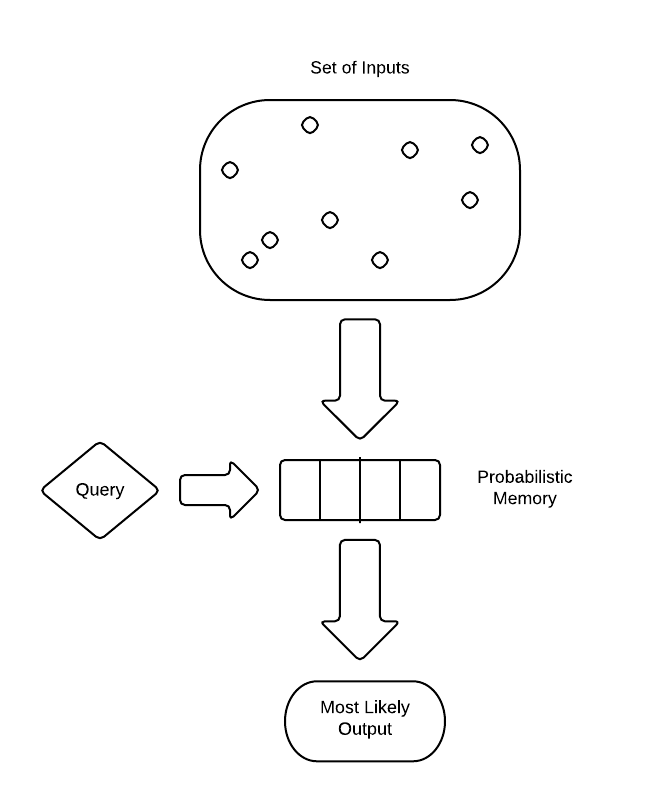
\includegraphics[width=1\linewidth]{pammodel}
%%	\end{center}
%%	\vspace{-12pt}
%%	\caption{Model of Probabilistic Associative Memory Mechanism}
%%	\label{fig:pammodel}
%%\end{figure}
%
%Perhaps a very significant source of complexity would come from evaluating
%queries, which raises the question
%of how they may be implemented. 
%As a simple example, queries for matching strings can be implemented in varying 
%degrees of complexity - from simple literal matching, to edit distance matching, 
%to even meaning analysis. For generic datatypes, as supported in this presented
%library, the issue becomes much more difficult. We anticipate requiring user
%input in order to determine how to calculate similarity, much like how 
%supervised machine learning algorithms require features to be decided. 
%While this does
%introduce an extra requirement for use, it will allow easy integration with
%structured data such as lists or trees. Alternatively, a form of feature
%selection may be useful, although usefulness may be limited without knowledge
%of the data type. 
%
%After the design stage, we will implement various types of probabilistic associative memories.
%An initial example implementation of the interface may be a deterministic version that
%ensures fidelity and keep track of every value that
%was stored in it. Later implementations will try to conserve memory space,
%and compress the stored values. We will work on several different data representation methods,
%including those related to neural networks. 
%
%By creating this interface, users of this programming language will be able to
%choose the type of memory and probabilistic model that most suits the needs of their particular
%application. Moreover, it will allow users to implement the interface with their own models as necessary, 
%as well as provide easy usage of the provided probabilistic models (Figure 2).

%\begin{figure}[H]
%	\begin{center}
%		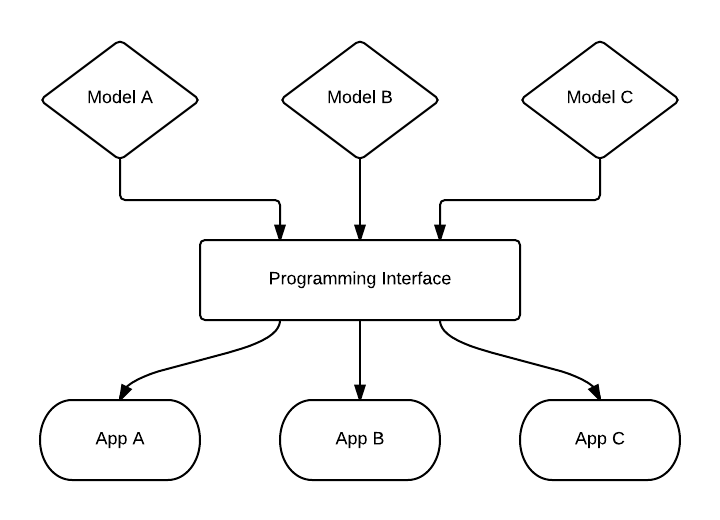
\includegraphics[width=1\linewidth]{block2}
%	\end{center}
%	\vspace{-12pt}
%	\caption{Programming Pipeline of our Library}
%	\label{fig:block2}
%\end{figure}

%The foremost technical challenges in our project involve creating the programming interface,
%the logistics of incorporating probabilistic models into the memory mechanism, and
%the mathematics involved in these models.
%
%Regarding the interface that the end user (programmer) sees, she should not have to be aware of 
%the inner workings of each probabilistic model, but expect reasonable and intuitive return values
%to each query into the probabilistic memory. For instance, if she is prioritizing accuracy 
%in her use of the library, she would expect a return value that was previously inserted and that 
%returns the highest probability for the given query.
%
%However, it is also necessary to give the programmer enough power and flexibility with our library for 
%whatever probabilistic applications she will be using it for. This involves enabling 
%her to create query combinations and queries of different types. Still, flexibility may 
%come at the cost of complexity - implementing features to accommodate arbitrary data, queries,
%and probabilistic models quickly increases the complexity of this project. 
%
%Regarding mathematics, it is necessary to further research mathematical 
%and probabilistic methods that would be implemented in this library. After implementing these methods,
%we will need to verify that mathematical or probabilistic models behave as expected. 
%For instance, if the previous values inserted into a high-fidelity probabilistic memory were ``cat, dog, mouse, horse", and we queried for an entry that best
%matches ``mousse", 
%then the expected return value would be ``mouse", since ``mouse" is the word most
%similar to our input. 
%Of course, in our actual implementation, we will have more complicated mechanisms than the one above. Perhaps the correct answer should not be ``mouse" depending
%on how the user defines similarity. 
%Thus, another challenge involves testing that our return values achieve a certain standard of accuracy or fidelity.
%
%\subsection{Evaluation Criteria}
%\label{subsec:eval_criteria}
%There are two main criteria which, combined, makes this library novel and effective. 
%The first criterion is that it provides comparable results to other associative memory techniques. 
%For instance, an autocomplete program (of sentences) can be written with this library and compared against an existing implementation of autocompletion. 
%Evaluating the correctness and results of these autocompletion programs may involve taking a collection of existing sentences and truncating them
%at certain places. First, a set of training data along with the truncated sentences will be passed into both autocompletion programs. 
%Then, the percentage of words that each program autocompleted correctly will be returned as the evaluation metric. 
%
%The second criterion, which is the main focus of the library, involves simplifying the programming interface for associative memory techniques.
%To evaluate this criterion, we will analyze how generic our code is. That is, given an autocompletion program, suppose one wanted to adapt this 
%program for recognizing a melody based only on a musical fragment or phrase. Ideally, the library would facillitate minimal changes to the existing 
%autocompletion program. The user would only need to provide different functions for evaluating the data, and the rest of the framework can remain as it is. 
%
%The utility of this library lies in its generality in implementing associative memory techniques. While this project does not attempt to improve 
%existing associative memory algorithms, it seeks to provide a simple, flexible interface for implementing associative memory applications.


% We next move onto the bibliography.
\bibliographystyle{plain} % Please do not change the bib-style
\bibliography{progress_spec}  % Just the *.BIB filename
\cite{holographic}
% Here is a dirty hack. We insert so much vertical space that the
% appendices, which want to begin in the left colunm underneath
% "references", are pushed over to the right-hand column. If we looked
% hard enough, there is probably a command to do exactly this (and
% wouldn't need tweaked after edits).
\vspace{175pt}

\end{document} 

